%%%%%%%%%%%%%%%%%%%%%%%%%%%%%%%%%%%%%%%%%%%%%%%%%%%%%%%%%%%%%%%%%%%%%
%
%  This is a sample LaTeX input file for your contribution to 
%  the MC2013 conference. Modified by R.C. Martineau at INL from A. 
%  Sood at LANL, from J. Wagner ORNL who obtained the original class 
%  file by Jim Warsa, LANL, 16 July 2002}
%
%  Please use it as a template for your full paper 
%    Accompanying/related file(s) include: 
%       1. Document class/format file: mc2013.cls
%       2. Sample Postscript Figure:   figure.eps
%       3. A PDF file showing the desired appearance: template.pdf 
%    Direct questions about these files to: richard.martinea@inl.gov
%
%    Notes: 
%      (1) You can use the "dvips" utility to convert .dvi 
%          files to PostScript.  Then, use either Acrobat 
%          Distiller or "ps2pdf" to convert to PDF format. 
%      (2) Different versions of LaTeX have been observed to 
%          shift the page down, causing improper margins.
%          If this occurs, adjust the "topmargin" value in the
%          mc2013.cls file to achieve the proper margins. 
%
%%%%%%%%%%%%%%%%%%%%%%%%%%%%%%%%%%%%%%%%%%%%%%%%%%%%%%%%%%%%%%%%%%%%%


%%%%%%%%%%%%%%%%%%%%%%%%%%%%%%%%%%%%%%%%%%%%%%%%%%%%%%%%%%%%%%%%%%%%%
\documentclass{ansconf}
%
%  various packages that you may wish to activate for usage 
\usepackage{graphicx}
\usepackage{tabls}
\usepackage{hyperref}
%

%General Short-Cut Commands
\newcommand{\superscript}[1]{\ensuremath{^{\textrm{#1}}}}
\newcommand{\subscript}[1]{\ensuremath{_{\textrm{#1}}}}
%\newcommand{\nuc}[2]{\superscript{#2}{#1}}
\newcommand{\nuc}[2]{{#1}{#2}}
\newcommand{\ith}[0]{$i^{\mbox{th}}$ }
\newcommand{\jth}[0]{$j^{\mbox{th}}$ }
\newcommand{\kth}[0]{$k^{\mbox{th}}$ }
\newcommand{\us}[0]{$\mu$s }

% New definition of square root:
% it renames \sqrt as \oldsqrt
\let\oldsqrt\sqrt
% it defines the new \sqrt in terms of the old one
\def\sqrt{\mathpalette\DHLhksqrt}
\def\DHLhksqrt#1#2{%
\setbox0=\hbox{$#1\oldsqrt{#2\,}$}\dimen0=\ht0
\advance\dimen0-0.2\ht0
\setbox2=\hbox{\vrule height\ht0 depth -\dimen0}%
{\box0\lower0.4pt\box2}}



% Insert authors' names and short version of title in lines below
%
\authorHead{Anthony M. Scopatz}
\shortTitle{First \& second order approximations to stage numbers in symbolic 
            multicomponent enrichment}

\confTitle{International Conference on Mathematics and Computational Methods
  Applied to Nuclear Science \& Engineering (M\&C 2013)}
\confLocation{Sun Valley, Idaho, USA, May 5-9, 2013}
\confPublished{on CD-ROM, American Nuclear Society, LaGrange Park, IL (2013)}

%%%%%%%%%%%%%%%%%%%%%%%%%%%%%%%%%%%%%%%%%%%%%%%%%%%%%%%%%%%%%%%%%%%%%
%
%   BEGIN DOCUMENT
%
%%%%%%%%%%%%%%%%%%%%%%%%%%%%%%%%%%%%%%%%%%%%%%%%%%%%%%%%%%%%%%%%%%%%%
\begin{document}

\title{FIRST \& SECOND ORDER APPROXIMATIONS TO STAGE NUMBERS IN SYMBOLIC 
       MULTICOMPONENT ENRICHMENT}

\author{Anthony Scopatz}
\affil{The University of Chicago\\
  5754 S. Ellis Ave, Chicago, IL, 60637 \\
  scopatz@flash.uchicago.edu}

\maketitle

\begin{abstract}
\raggedright
Some Abstract text.

\emph{Key Words}: multicomponent, enrichment, symbolic, PyNE
\end{abstract}

\section{Introduction}
\label{sec:intro}

The matched abundance ratio equations which are used to compute concentrations and 
flow rates through a multicomponent enrichment cascade contain a number of terms 
proportional to the number components.  While the number of components may be 
handled elegantly mathematically, computing a greater number of components 
penalizes anyone (human or computer) actually performing the 
calculation.  However, 
symbolic expression codes are capable of closely matching the original 
mathematical representation of the cascade equations.

A variety of symbolic mathematics software tools exist. Examples include  
Mathematica \cite{Wolfram2008}, Maple \cite{Maple16},  Maxima \cite{Maxima5}, 
and SymPy \cite{SymPy2012}.  These codes excel at abstract representation and 
manipulation of mathematical symbols.  Even complicated operators such as 
differentiation and integration may be represented or applied as desired by the 
user.  Therefore solving systems of equations with symbolic computational tools
has been possible since the 1980s.

Where such codes tend to fall short is during numeric evaluation of 
their symbolic expressions.  While acceptable performance is seen 
for small to medium numbers of 
operations, they have difficulty scaling to large computations.  Moreover, 
numeric, vectorized, or compiled expressions will always be executed faster
by the processor.  Part of the blame may lie with the fact that the some symbolic 
libraries evaluate their 
expressions with arbitrarily large floating point precision.  (Numeric libraries
typically deal in fixed precision, normally 64-bits on modern systems.)  However, 
float evaluation of a symbolic expression is more likely slow because an entire 
tree of sub-expressions must be walked and evaluated to produce the final result.

Slow numeric evaluation is what prevents symbolic tools from being used at a 
production level.  Rather such tools fill the niche of demonstrating that a new
method works prior to writing a numeric implementation.  To aid in this 
process some symbolic libraries, such as Mathematica and SymPy, now include
code generation features.  These routines will convert symbolic expressions into
C, Fortran, or Python code.  For Mathematica, this is still not a perfect solution
because the generated code may call back to the symbolic library for certain 
sub-expressions.

Still, code generation from symbolic expressions provides an interesting opportunity. 
It enables a workflow 
where the symbolic expressions for a system of equations are manipulated, solved, 
reduced to a minimal form, used to produced machine code, and finally executed by
the user.  Since only this last step is present at run time, everything else in this
pipeline is effectively a pre-processing step.  While this pre-processing might be 
computationally expensive it will not affect the final run times.  If this
process is implemented correctly, and efficient code is generated, than these 
final run times may be quite fast.

Of interest are the matched abundance ratio cascade (MARC) equations for 
multicomponent separations originally described by de la Garza \cite{DelaGarza1969}.
This system may be solved using a constrained numerical optimizer 
\cite{doi:10.1080/01496391003793884,pyne:enrichment}.  These equations make for an
exciting challenge since some of the independent variables cannot be exactly
expressed as a closed form function of the other independent variables. 
Furthermore, closed form approximations are typically not used because 
there are too many terms to mange by hand.  Thus, numeric optimizers have been used 
to solve the MARC equations for the all independent variables simultaneously.

Alternatively, a symbolic mathematics library is able to supervise expressions 
with many orders of magnitude more terms than a human may handle.  Therefore
implementing closed form expressions for all independent variables is now a realistic 
possibility.  From here, solving the MARC system of equations may take place via
variable substitution and elimination.
Coupled with code generation techniques, this paper explores symbolic solutions 
that are at least as accurate and have faster execution times than numerical solvers.

Both the symbolic and the numeric MARC solvers discussed here are part of the free 
\& open source computational nuclear engineering toolkit PyNE \cite{PyNE2012}.  
The reader may therefore inspect the implementation of both methods at will.
SymPy was used as the symbolic mathematics library because 
it offered the most flexibility with respect to code generation.

The remainder of this document proceeds as follows.  The symbolic methodology 
is discussed in \S\ref{sec:meth}.  This includes an overview of the
MARC equations, a detailed explanation of the symbolic strategy used to solve 
them, and a full description of the code generation pipeline.
Results are then presented in \S\ref{sec:res}.  This includes multiple benchmarks
with to an alternative numeric solver as well as to published cascade results by other 
authors.  Finally, \S\ref{sec:conc} discusses the validity of the presented method
as well as possible avenues for further research.

\section{Symbolic Methodology}
\label{sec:meth}
At its core, the solution to coupled multicomponent enrichment cascade equations is
a minimization problem \cite{Wood1999}.  In a matched abundance ratio 
\cite{DelaGarza1969} cascade this may be cast as the minimization of 
the total flow rate $L$ through the cascade normalized by the feed flow rate $F$.  
Thus, the positive and unitless optimization variable $L/F$ is formed.  Traditionally, 
minimizing this parameter as a function of other cascade state variables has been 
performed either via off-the-shelf optimization libraries 
\cite{doi:10.1080/01496391003793884} or custom built solvers \cite{PyNE2012}.

However, both of these approaches rely on writing code idiomatic to the underlying 
programming language.  For example, many numerical constraint optimizers, in order 
to handle the case of arbitrarily complex expressions, accept as their primary 
argument a function object or pointer.  Then for every iteration the optimizer must 
call the function whose inputs are to be optimized.  This involves (in compiled 
languages) setting up a new stack and allocating new memory for every solver 
iteration.  While good 
optimizers will be efficient in terms of the number of function calls they make, 
there is no way for them to avoid multiple function calls and remain sufficiently 
general. The number of function calls that are needed scales \emph{at least} linearly 
with the number of equations in the system.

On the other hand, if it is possible to convert the system of equations 
into a single expression -- no matter how complicated -- then the problem has been 
recast into the optimization of a single function over a single variable.   This 
may be easily handed off to any number of well known algorithms, such as Newton's
method, the secant method, or the bisection method.  In such a form, the solution 
will have a vastly reduced computational overhead as compared to standard 
numerical solvers. 

Naturally, performing the above variable substitution and elimination to obtain a 
single expression is difficult in many cases and mathematically impossible in most 
others.  For MARC systems, as is shown in \S \ref{sec:symes}, reduction of $L/F$
to a single expression is possible.

Rather than phrasing this as a numerical optimization problem from the start, the 
opposite conceptual tactic is taken.  The MARC system is expanded, manipulated, 
and substituted symbolically during the majority of the calculation.  The actual 
numerical results of the calculation are only computed as needed at the final step.
Symbolic manipulations are concluded prior to compilation, resulting in 
very fast run time solutions.

In \S \ref{sec:marceq} the standard MARC system of equations is detailed. 
Then the novel reinterpretation of the MARC equations is related in 
\S \ref{sec:symes}.  
Lastly, \S \ref{sec:codegen} characterizes the pipeline that takes the symbolic MARC 
equations and converts them into fast machine code.  
For the remainder of \S \ref{sec:meth}, a three-component natural uranium fed 
cascade will be used when example data is required.
Cascades with a greater numbers of components will be discussed in \S \ref{sec:res}.

\subsection{The MARC Equations}
\label{sec:marceq}
The method to compute matched abundance ratio cascades has been 
previously described in other sources, from de la Garza in the
1960s. This method is explained here in order to build up to the symbolic first and 
second order approximations that will be seen.
For more information please refer to de la Garza
\cite{DelaGarza1969}, von Halle \cite{VonHalle1987}, Wood \cite{Wood1999}, 
Song \cite{doi:10.1080/01496391003793884}, or the symbolic methodology on which this 
work is based \cite{Scopatz2012}.

Set $N$ the total number of stages in an enrichment cascade, $N_P$ as the number of 
product stages above the feed entry point, and $N_T$ as the number of tails
stages.  Thus,
\begin{equation}
N = N_P + N_T
\end{equation}
MARC needs a special nuclide to also be set such that it is enriched in the 
product (subscript P).  This is called the first key component, $j$.  
There is also be a second key component, $k$, from which $j$ is 
separated. Therefore $k$ can be said to be enriched in the tails stream (subscript T).

The overall stage separation factor $\alpha$ [unitless] is the per mass 
enrichment ratio from one stage to the next.  From $\alpha$ 
stage separation factors for individual nuclides may be computed. 
These are called $\beta_i$ for the \ith component of a mixture $I$ and are 
computed by:
\begin{equation}
\beta_i = \alpha^{M^* - M_i}
\label{beta_i}
\end{equation}
$M_i$ is the molecular weight [amu] of the \ith
nuclide while $M^*$ [amu] is a flow rate optimization parameter.  An initial
guess for 
$M^*$ is normally set by the average of the molecular weights of the key components. 
Using the subscript $0$, denote the initial guess by $M_0^*$:
\begin{equation}
M_0^* = \frac{1}{2}\left(M_j + M_k\right)
\label{mstar-guess}
\end{equation}
Also the constraint $M_j < M_k$ is applied when picking the order for$j$ \& $k$.
Thus $M^*$ is bounded on the range $M^*\in[M_j,M_k]$ when minimizing $L/F$.

Call $F$, $P$, and $T$ the feed, product, and tails mass flow rates subject to 
the conservation equation,
\begin{equation}
F = P + T
\label{total-flow-constraint}
\end{equation}
Also have $x$ as a normalized mass concentration vector such that $x_i^F$, 
$x_i^P$, $x_i^T$ are the concentrations of the \ith nuclide of the feed, product,
and tails.  From here:
\begin{equation}
1 = \sum_i^I x_i^F = \sum_i^I x_i^P = \sum_i^I x_i^T 
\end{equation}
The flow rate ratios are seen as follows:
\begin{equation}
\frac{P}{F} = \sum_i^I x_i^F\frac{\beta_i^{N_T+1} - 1}
                                 {\beta_i^{N_T+1} - \beta_i^{-N_P}}
\label{ppf-full}
\end{equation}
\begin{equation}
\frac{T}{F} = \sum_i^I x_i^F\frac{1 - \beta_i^{-N_P}}
                                 {\beta_i^{N_T+1} - \beta_i^{-N_P}}
\label{tpf-full}
\end{equation}
Equations \ref{ppf-full} \&  \ref{tpf-full} are then reduced to functions
of just $j$ for an ideal cascade.
\begin{equation}
\frac{P}{F} = \frac{x_j^F - x_j^T}{x_j^P - x_j^T}
\label{ppf-key}
\end{equation}
\begin{equation}
\frac{T}{F} = \frac{x_j^F - x_j^P}{x_j^T - x_j^P}
\label{tpf-key}
\end{equation}

Equations \ref{ppf-full} \& \ref{tpf-full} or equations \ref{ppf-key} \& 
\ref{tpf-key} both allow for the calculation of the \ith component concentrations in 
the product and tails as a function of the feed concentrations.
\begin{equation}
x_i^P = \frac{x_i^F}{\frac{P}{F}}\cdot\frac{\beta_i^{N_T+1} - 1}
                                           {\beta_i^{N_T+1} - \beta_i^{-N_P}}
\label{prod-concentration}
\end{equation}
\begin{equation}
x_i^T = \frac{x_i^F}{\frac{T}{F}}\cdot\frac{1 - \beta_i^{-N_P}}
                                           {\beta_i^{N_T+1} - \beta_i^{-N_P}}
\label{tail-concentration}
\end{equation}
However, the component nuclides themselves are
also subject to mass conservation:
\begin{equation}
x_i^FF = x_i^PP + x_i^TT
\label{comp-flow-constraint}
\end{equation}

By their name, MARCs require that at every stage any two flows of 
the same type ($F$, $P$, \& $T$) must have the same relative concentrations of 
$j$ \& $k$.  Thus, say that $R$ is an abundance ratio.  For matched abundance 
ratio cascades, 
\begin{equation}
R^F = \frac{x_j^F}{x_k^F}; \;\;\; R^P = \frac{x_j^P}{x_k^P}; \;\;\; 
R^T = \frac{x_j^T}{x_k^T}
\label{abund_ratios}
\end{equation}
The ratios in these equations are valid for all stages in the cascade.

Lastly, the total flow rate per $F$ for a cascade is computed as follows:
\begin{equation}
\frac{L}{F} = \sum_i^I \frac{\frac{P}{F}x_i^P\ln(R^P) + \frac{T}{F}x_i^T\ln(R^T) 
                                                      - x_i^F\ln(R^F)}
                            {\ln(\beta_j)\frac{\beta_i - 1.0}{\beta_i + 1.0}}
\label{ltot-over-feed}
\end{equation}
Equation \ref{ltot-over-feed} is minimized when computing the `optimal' cascade.
This is analogous to the $L/P$ expression found in \cite{Wood1999}.

Typically, the following cascade parameters are known:
$\alpha$, 
$j$, $k$, 
$M_i$ for all $i\in I$, 
$x_i^F$ for all $i\in I$, 
the key product enrichment $x_j^P$, and the key 
tails enrichment $x_j^T$.  Therefore the optimized cascade is given by 
a system of three equations and three unknowns --
$N_P$, $N_T$, and $M^*$ -- and is therefore well determined.
\begin{equation}
\frac{x_j^P}{x_j^F}\cdot\frac{P}{F} - \frac{\beta_j^{N_T+1} - 1}
                                           {\beta_j^{N_T+1} - \beta_j^{-N_P}} = 0
\label{prod-constraint}
\end{equation}
\begin{equation}
\left(\frac{x_j^F}{\frac{T}{F}} \cdot \frac{1 - \beta_i^{-N_P}}
                                           {\beta_j^{N_T+1} - \beta_j^{-N_P}} \right)
- \left(x_j^T\cdot\sum_i^{I} x_i^T\right) = 0
\label{tail-constraint}
\end{equation}
\begin{equation}
\min\left[\frac{L}{F}\right]\to \frac{d}{dM^*} \frac{L}{F} = 0
\label{minlt-constraint}
\end{equation}
Equation \ref{prod-constraint} is a rearrangement of equation \ref{prod-concentration}
when evaluated for the second key component.
Equation \ref{tail-constraint} is gained by equations \ref{tpf-full} \&
\ref{tail-concentration} when evaluated for the second key component.
Equation \ref{minlt-constraint} comes from the extreme value theorem of calculus
and equation \ref{ltot-over-feed}.

\subsection{Symbolic Enrichment Solver}
\label{sec:symes}

When solving a system of equations, it is advantageous if any of the independent 
variables has a closed form representation in terms of the other independent 
parameters. This is because the closed form solution may be substituted into 
the remaining equations and this variable eliminated from the computation.  This
transforms the system from $X$ equations with $X$ unknowns into a system with 
$(X-1)$ equations and $(X-1)$  unknowns.  Ideally, the system is reducible 
to one equation as a function of one unknown, having potentially undergone many 
substitutions.

The symbolic MARC algorithm here relies on eliminating the $N_P$ and $N_T$ variables
from equations \ref{prod-constraint}-\ref{minlt-constraint}. This produces a single
expression for $L/F$, which may be handed to a traditional minimization algorithm.
Thus, the strategy for engineering a successful symbolic solver for a given system
of equations is distinct from the normal numeric mechanisms.

Unlike numeric solvers where every expression is evaluated with an integer, real, or
complex number as it is encountered, symbolic computation represents and stores all 
operations performed on an expression.  Only after the accumulation of all 
operations -- and only if desired by the user -- is a symbolic expression ever numerically
evaluated.  This is true even for compound operators such as trigonometric functions, 
differentiation, and integration.

Hence certain operators may explode the number of binary
operations in the resultant expression after their application. 
(For example, the chain rule for differentiation may have many more terms that 
the original function.)
So while the quintessential strategy in numerical solvers is to mitigate error
stemming from floating point arithmetic, a symbolic solver seeks to minimize the total
number of irreducible operations ($+, -, \times, /, \%, \log, \sin, \mbox{abs},$ etc.). 
Therefore much of the variable
elimination below also attempts to simultaneously curtail the overall operation count. 

Start by considering the constraint in equation \ref{prod-constraint}, the key 
component simplification of $P/F$ seen in equation \ref{ppf-key}, and the number
of tails stages $N_T$.  A call to SymPy's \texttt{solve()} function rearranges the 
constraint to reveal the closed form solution $N_T(N_P, M^*)$:
\begin{equation}
\begin{array}{lcl}
N_T & = & \left[- M^{*} N_{P} \log{\left (\alpha \right )} - M^{*} \log{\left (\alpha \right )} + M_{j} \log{\left (\alpha \right )} - \log{\left (x^{T}_{j} \right )} \right. \\ 
& & \left. - \log{\left (\frac{- x^{F}_{j} + x^{P}_{j}}{\alpha^{M^{*} N_{P}} x^{F}_{j} x^{P}_{j} - \alpha^{M^{*} N_{P}}x^{F}_{j} x^{T}_{j} - \alpha^{M_{j} N_{P}} x^{F}_{j} x^{P}_{j} + \alpha^{M_{j} N_{P}} x^{P}_{j} x^{T}_{j}} \right )} \right] \\
& & \times \left[\left(M^{*} - M_{j}\right) \log{\left (\alpha \right )} \right]^{-1}
\end{array}
\label{nt_closed_full}
\end{equation}
While equation \ref{nt_closed_full} is only a function of known 
parameters, $N_P$, and $M^*$, it is not an exemplary expression.  This is because both 
$M^*$ and $N_P$ each appear five times in this closed form solution.  Thus if this 
were substituted into the original MARC system to eliminate $N_T$, the number of 
instances of independent variables would grow by a ratio of 10:1.    

To decrease the substitution ratio and simplify the expression, equation 
\ref{nt_closed_full} may be rewritten (by hand) as the following:
\begin{equation}
\begin{array}{lcl}
N_T & = & \left[M^{*} \log{\left (\alpha \right )} - M_{j} \log{\left (\alpha \right )} + \log{\left (x^{T}_{j} \right )} + \log{\left (\frac{-1.0 + \frac{x^{P}_{j}}{x^{F}_{j}}}{x^{P}_{j} - x^{T}_{j}} \right )}  \right. \\
& & \left. - \log{\left (\frac{\alpha^{N_{P} \left(- M^{*} + M_{j}\right)} \left(x^{F}_{j} x^{P}_{j} - x^{P}_{j} x^{T}_{j}\right)}{- x^{F}_{j} x^{P}_{j} + x^{F}_{j} x^{T}_{j}} + 1 \right )}\right] \times \frac{1}{\left(- M^{*} + M_{j}\right) \log{\left (\alpha \right )}} \\
\end{array}
\label{nt_closed}
\end{equation}
Note that this transformation requires the logarithm identity 
$\log(a+c) = \log(a) + \log(1 + \frac{c}{a})$.  Equation \ref{nt_closed} is superior
in the sense that it requires 31 operations to as opposed to the original 38.
More importantly, $N_P$ appears only once in this 
expression and $M^*$ is reduced to three occurrences.

\begin{figure}[htpb]
\begin{center}
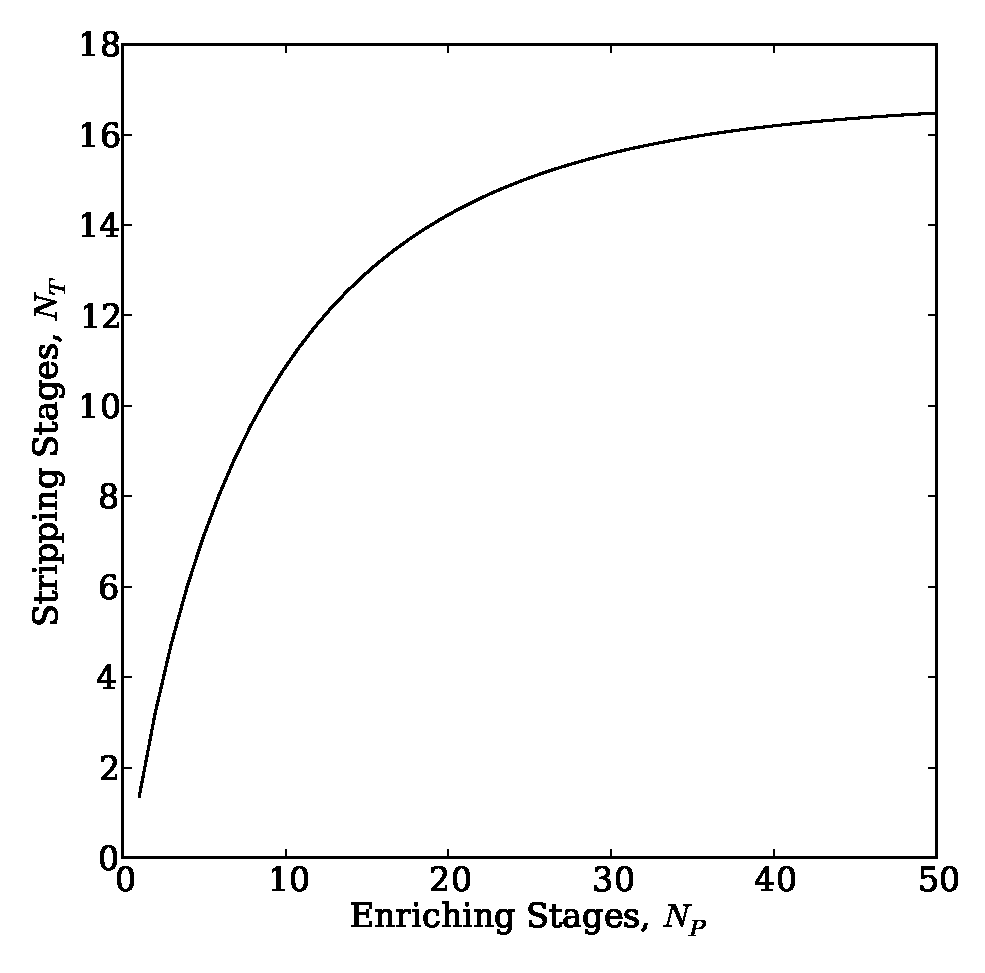
\includegraphics[scale=0.5]{nt_closed.eps}
\caption{$N_T(N_P, M^*)$ for a natural uranium cascade with $N_P\in[1,50]$ and 
    $M^*=236.547$.}
\label{nt_closed_fig}
\end{center}
\end{figure}

Figure \ref{nt_closed_fig} confirms that the closed form $N_T(N_P, M^*)$ is correct.
For an increasing number of enriching stages, the stripping stages must also 
increase to maintain the proper mass flow rates.
This figure was computed 
with the feed concentrations seen in Table \ref{feed_nu} and the following other 
cascade parameters: $M^*=236.547$, $N_P^0=30$, $N_T^0=10$, $\alpha=1.05$, 
\nuc{U}{235} as the \jth key component, \nuc{U}{238} as the \kth key component, 
$x_j^P=0.055$, and $x_j^T=0.0025$.
Therefore, equation \ref{nt_closed} allows for the elimination of $N_T$ as an 
independent variable when computing $L/F$ and $N_P$.  

\begin{table}[htbp]
\begin{center}
\caption{Feed flow concentrations for a natural uranium cascade.}
\include{feed_nu}
\label{feed_nu}
\end{center}
\end{table}

Next, examine the MARC constraint in equation \ref{tail-constraint}.  This states that
the tails concentration of the \jth key component that is computed by the concentration
equations \emph{must} be equal to the concentration specified for the cascade in the
initial conditions.  (Recall that $x_j^T$ is one of the known parameters.)  
Substituting $N_T(N_P, M^*)$ into this expression, the function $f$ is obtained:
\begin{equation}
f(N_P,M^*) =
\left(\frac{x_j^F}{\frac{T}{F}} \cdot \frac{1 - \beta_i^{-N_P}}
                                           {\beta_j^{N_T(N_P,M^*)+1} - \beta_j^{-N_P}} \right)
- \left(x_j^T\cdot\sum_i^{I} x_i^T\right) \equiv 0
\end{equation}
Here again, like with $P/F$ above, the key component simplification of $T/F$ in 
equation \ref{tpf-key} is used.

It would be highly valuable if the terms in $f(N_P,M^*)$ were rearrangeable into 
a closed form expression
for either $N_P$ or $M^*$.  Since there are fewer instances of $N_P$, the number of
enriching stages would be the preferred candidate.  However from Galois theory, 
due to structure of $f(N_P,M^*)$ no such closed form solution is possible.  Examining
with respect to just $N_P$, the structure of $f$ roughly fits:
\begin{equation}
\frac{1 + \alpha^{-N_P}}{\alpha^{-\log(\alpha^{-N_P})+1} - \alpha^{-N_P}} - x_j^T
    \frac{1 + \alpha^{-N_P}}{\alpha^{-\log(\alpha^{-N_P})+1} - \alpha^{-N_P}} -
    \cdots 
\end{equation}
Even this overly simplified representation cannot be rearranged as is to give a 
closed form function for $N_P$.  It may be possible to achieve such an expression 
by making logarithm approximations, such as $\log(a) \approx a - 1$ for $a\approx1$.  
This could 
eliminate the nested powers of $N_P$ which would potentially yield
a closed form representation.  However, since the $\log$ terms appear in the exponent
of $\alpha$, any error induced by these approximations would be compounded 
unnecessarily.  Therefore this line of inquiry was not pursued further.

\begin{figure}[htpb]
\begin{center}
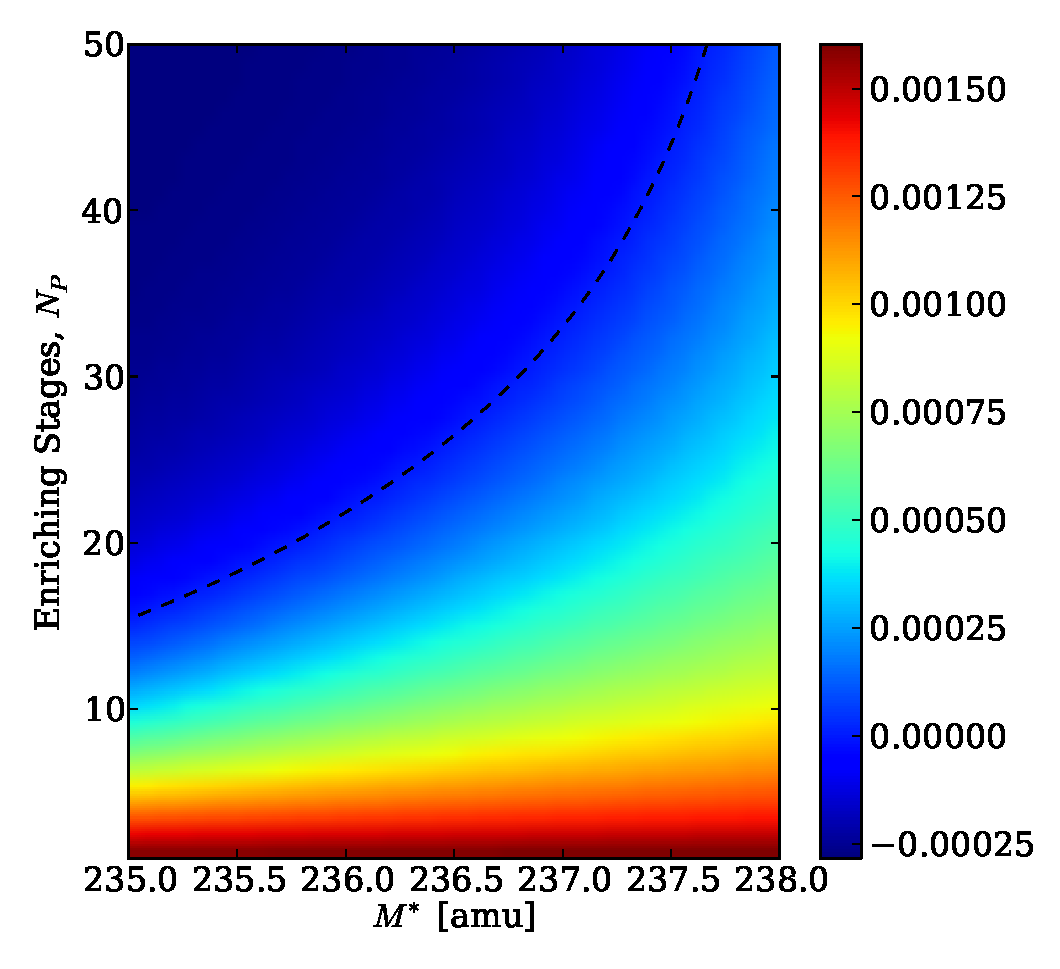
\includegraphics[scale=0.5]{np_constraint.eps}
\caption{$f(N_P, M^*)$ over the range of possible $N_P$ and $M^*$ values.  The black
contour line represents $f(N_P, M^*)=0$ and is the solution to the MARC constraint
in equation \ref{tail-constraint}. 
Data was computed for a typical natural uranium fed cascade.}
\label{np_constraint_fig}
\end{center}
\end{figure}

Instead, $f(N_P,M^*)$ was plotted as an unconstrained function of its two remaining 
independent variables to produce the heat map that may be seen in Figure 
\ref{np_constraint_fig}.  Since the range of $f$ contains both positive and negative
values, it follows that there must be some combination of $(N_P,M^*)$ which
satisfy the original MARC constraint.  This $f(N_P, M^*)=0$ set is displayed on Figure 
\ref{np_constraint_fig} as the black contour.  While this contour could hypothetically
be used itself to provide a closed form $N_P(M^*)$ equation, such a strategy would 
be grossly inefficient.  This is because a large number of $f$ points must be 
numerically evaluated, and then lineally interpolated, to fit such a curve with
respectable accuracy.

Rather, by inspection of Figure \ref{np_constraint_fig}, the $f(N_P, M^*)=0$ curve 
would be well fit by a second order polynomial on the domain of interest.
That the constraint follows this form is not obvious from either equation 
\ref{tail-constraint} or $f(N_P,M^*)$.  The coefficients in 
such a second order polynomial model cannot be precomputed  numerically and must be 
expressed symbolically in terms of known parameters and independent variables 
\cite{Sacks:1989:ASS:1623755.1623823}.

On this basis, represent $f$ by its second order Taylor series expansion with
respect to $N_P$ close to the initial guess $N_P^0$.
\begin{equation}
\begin{array}{rcl}
f(N_P,M^*) & \approx &f(N_P^0,M^*) \\
& & + \left(N_P -N_P^0\right)\left.\frac{df}{dN_P}\right|_{N_P=N_P^0} \\
& & + \frac{\left(N_P -N_P^0\right)^2}{2}\cdot\left.\frac{d^2f}{(dN_P)^2}\right|_{N_P=N_P^0}\\
\end{array}
\label{f-taylor}
\end{equation}
This may be refactored with the introduction of coefficients $a$, $b$, and $c$ into 
the canonical polynomial form,
\begin{equation}
\begin{array}{rcl}
f(N_P,M^*) & = & a(N_P)^2 + bN_P + c\\
a & = & \frac{1}{2}\cdot\frac{d^2f}{(dN_P)^2}\\
b & = & \left.\frac{df}{dN_P}\right|_{N_P=N_P^0} - N_P^0\frac{d^2f}{(dN_P)^2} \\
c & = & f(N_P^0,M^*) - N_P^0\cdot\frac{df}{dN_P} + \frac{(N_P^0)^2}{2}\frac{d^2f}{(dN_P)^2} \\
\end{array}
\label{f-cannon}
\end{equation}
where all derivatives in equation \ref{f-cannon} are evaluated at $N_P=N_P^0$.
Applying the constraint $f(N_P,M^*)=0$, 
a closed form expression $N_P(M^*)$ is trivially solved for via the 
quadratic equation.
\begin{equation}
N_P(M^*) = \frac{-b - \sqrt{b^2 - 4ac}}{2a}
\label{np_closed}
\end{equation}
Note that for this approximation $a$ is always positive, $b$ is always negative, 
and the discriminant inside the square root is always positive.  Therefore only the 
negative solution to the quadratic is needed to obtain a well-bounded result for
$N_P(M^*)$.

\begin{figure}[htpb]
\begin{center}
\begin{tabular}{cc}
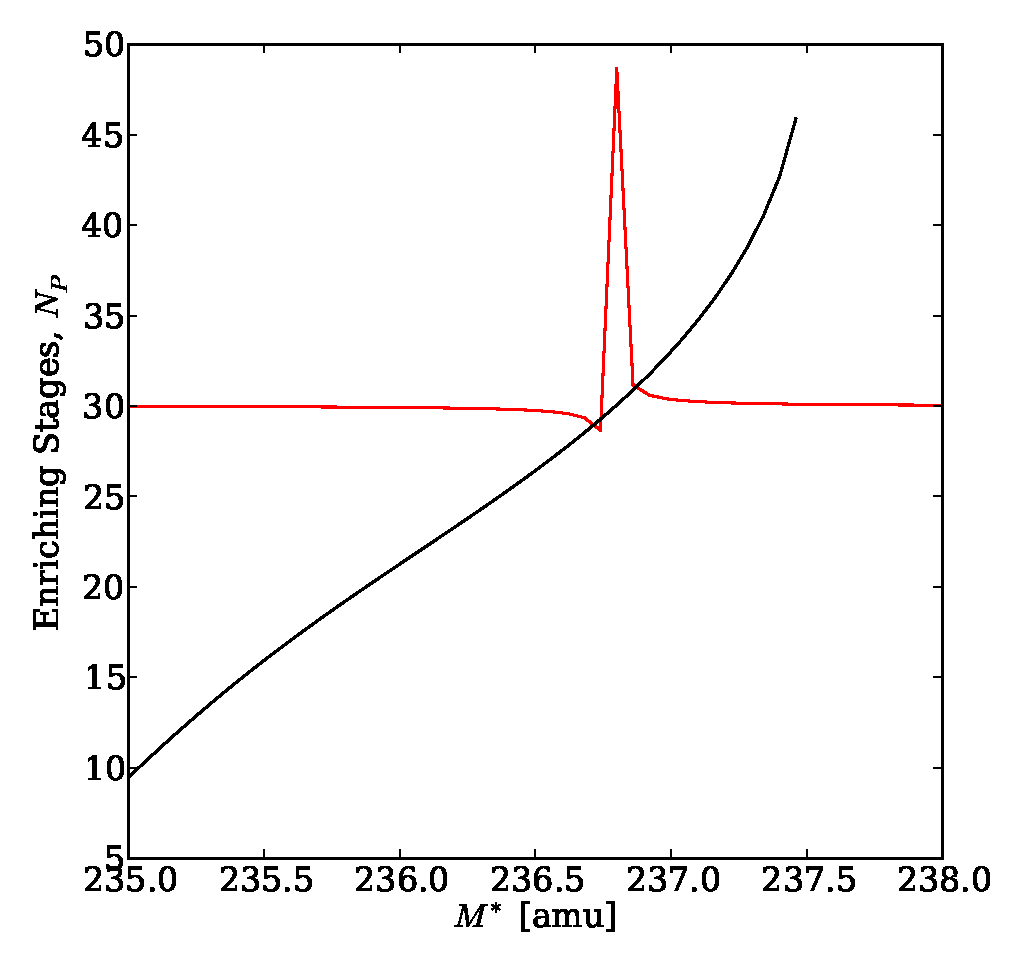
\includegraphics[scale=0.375]{np_closed.eps} & 
                                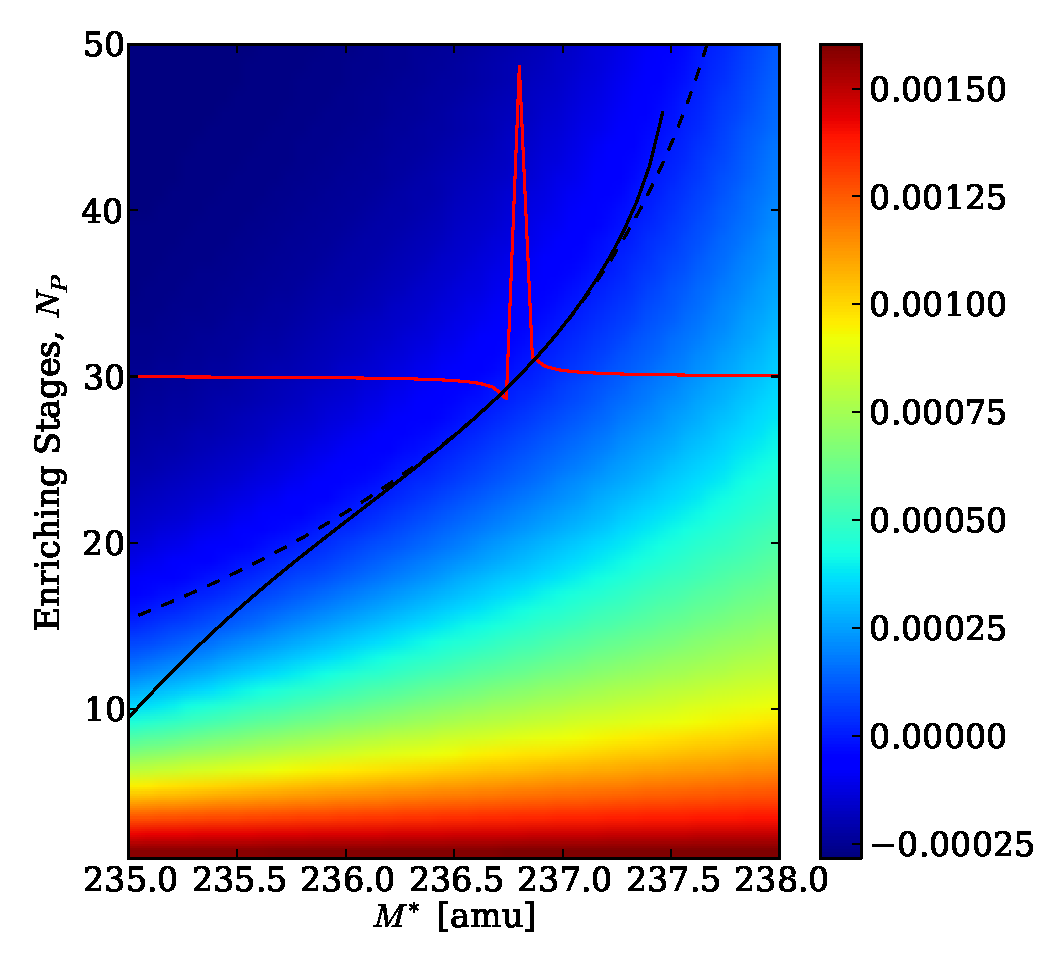
\includegraphics[scale=0.375]{np_closed_overlay.eps} \\
(a) & (b) \\
\end{tabular}
\caption{$N_T(M^*)$ such that $f(N_P,M^*)=0$.  (a): The quadratic solution to a
Taylor series approximation. This curve is truncated when negative discriminants 
would result in a complex solution.  (b): The equation from (a) as a dashed black 
line overlaid on top of Figure \ref{np_constraint_fig}.  The solid black line is a 
linearly interpolated contour for $f(N_P, M^*)=0$. The two sub-figures show that 
$N_P(M^*)$ is an accurate  approximation near the initial guesses $N_P^0$ and 
$M_0^*=(M_j+M_k)/2$, but less precise far from this point. Data was computed for 
a typical natural uranium fed cascade.}
\label{np_closed_fig}
\end{center}
\end{figure}

Figure \ref{np_closed_fig} plots the closed form solution to $N_P(M^*)$ both (a)
on its own and (b) overlaid onto the heat map in Figure \ref{np_constraint_fig}.  
This shows that the 
quadratic solution to the second order Taylor series approximation is an astoundingly 
accurate one when close to the initial conditions $N_P=N_P^0$ and $M_0^*=(M_j+M_k)/2$.
Naturally being only second order, this approximation breaks down farther away from 
the initial guess.  For greater values of $N_P$ and $M^*$, the curve begins to 
over-predict the result until the point that the discriminant becomes negative, the
solution becomes complex, and the data set is truncated.  For smaller values, the
result diverges by under-predicting.  That $N_P(M^*)$ deviates at the edges of the
domain is an expected phenomenon for Taylor series approximations.

\begin{figure}[htpb]
\begin{center}
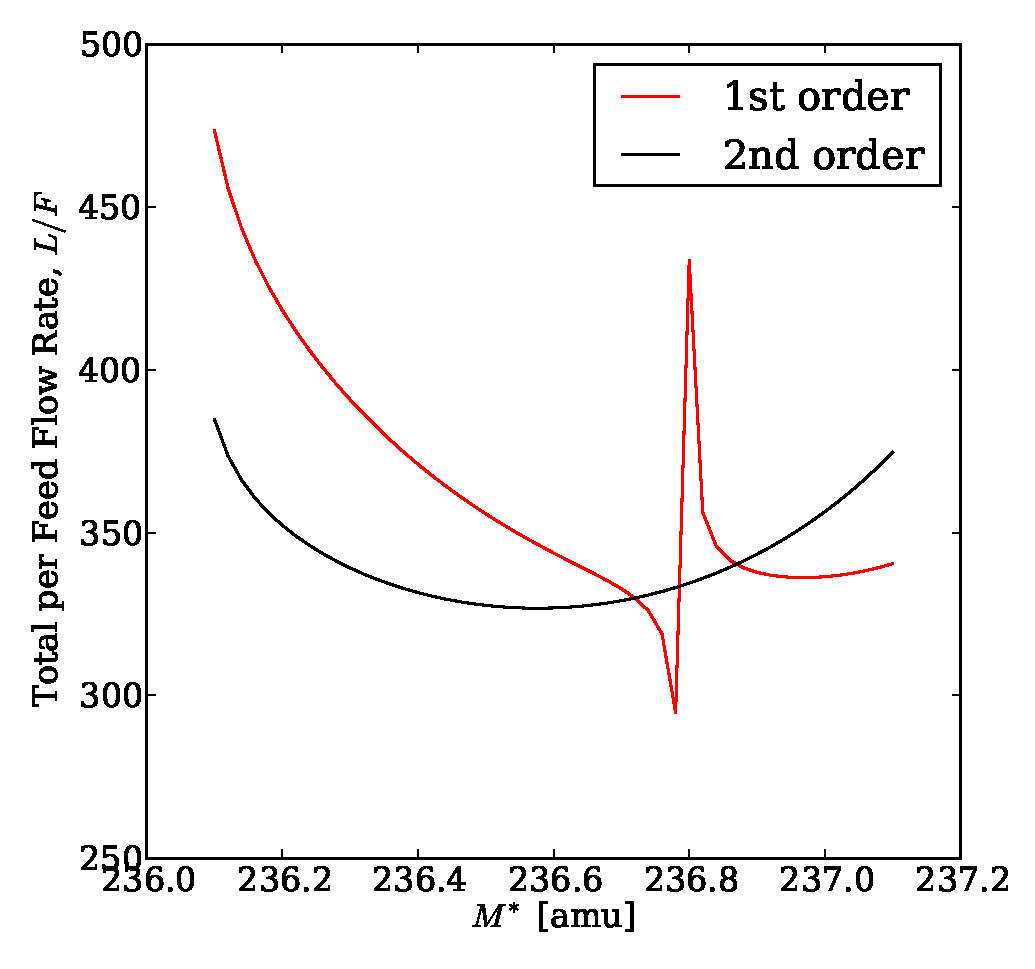
\includegraphics[scale=0.5]{loverf.eps}
\caption{$L/F(M^*)$ over the range of valid $M^*$ values.
Data was computed for a typical natural uranium cascade.}
\label{loverf_fig}
\end{center}
\end{figure}

Therefore, equation \ref{np_closed} may be substituted into equation \ref{nt_closed}
to obtain an expression $N_T(N_P(M^*),M^*)=N_T(M^*)$ which only depends on $M^*$ and 
the initial conditions.  Moreover, both equations \ref{nt_closed} \& \ref{np_closed}
may be substituted into equation \ref{ltot-over-feed} to obtain 
$L/F(N_P(M^*),N_T(M^*),M^*)=L/F(M^*)$ solely as a function of $M^*$.  Thus
$L/F(M^*)$ may be minimized using any standard one-dimensional algorithm.

Figure \ref{loverf_fig} shows $L/F(M^*)$ for the full domain of $M^*$, demonstrating 
that this symbolic methodology computes the correct bowl-like shape.  Note that while 
this method is successful, the number of operations in the final form of $L/T$ may be 
in the thousands to millions depending on how many components are included in the 
calculation.  A mechanism for mitigating huge numbers of operations is described
in \S \ref{sec:codegen}.


\section{Conclusions \& Future Work}
\label{sec:conc}

A symbolic multicomponent enrichment algorithm which is as or more accurate as 
standard numerical solvers has been demonstrated.  This new method is 20 - 300
times faster than its numeric counterpart, requiring run times on the order of 10 \us.
This may be used to calculate concentrations and flow rates.  It also may be used 
within an optimization algorithm to solve for $\min\left[L/F\right]$.

In essence, the symbolic solver is at least as accurate as numeric methods because
it maintains the mathematical relationships between terms for as long as possible.
It does not wash wash away these relationships by evaluating floating point data
until the last possible step.

Furthermore, this solution is significantly quicker to execute because it avoids
repeatedly using idiomatic language constructions which slow down computation (such
as function calls, loops, and heap memory).  Additionally, the symbolic solution is
passed through a common sub-expression elimination routine.  This further minimizes
the number of operations that are performed.  While this is done to some extent when 
hand-writing source code, a human is not capable of eliminating operations as 
thoroughly and error-free as an auto-generated solution.

Even with the very promising speed ups observed in the symbolic solver there are 
still areas for potential further improvement.  For example, the speed ups of the 
minimization of $L/F$ follow roughly linearly from the speed ups observed for the
underlying $L/F$ calculation.  However, the solution to $L/F(M^*)$ is known.
Therefore there is no theoretical reason why the $\min\left[L/F\right]$ step 
cannot be unrolled symbolically as well.

Suppose Newton's method was chosen to compute the minimum $M^*$.  Guessing 
an initial $M_0^*$, the optimization itself would be expressed symbolically as:
\begin{equation}
M^* = M_0^* - \frac{1}{L/F(M_0^*)}\left(\left.\frac{d}{dM^*}L/F(M^*)\right|_{M^*=M_0^*}\right)
\label{mstar-newton-min}
\end{equation}
While such a mechanism was explored for preparation of this study, the derivative
in this expression explodes the number of terms into the millions.  This far exceeds
the memory limitations of most individual computing resources.  

The term explosion in equation \ref{mstar-newton-min} is particularly problematic 
since most other optimization strategies require
even more derivatives to be evaluated.  So while symbolically minimizing $L/F(M^*)$
 promises
to decreases the execution time by perhaps another 10 - 100 times, it is 
outside the scope of contemporary compute resources without modifying the 
code generation algorithm.  Still, the symbolic minimization strategy detailed above
may be worth revisiting after another 5 - 10 years of computational evolution.

Instead, the impatient may decided to re-examine the code generation pipeline to 
produce more symbolic expressions faster.  Improvements here may open up the 
possibility of
a symbolic minimizer.  This could involve multiple smaller CSE passes.  How 
such code generation routines fit together remains as an open problem.

Another avenue for possible future research is the investigation of non-MARC 
systems.  Due to the speed of the symbolic solver, the abundance ratios for 
each centrifuge in a stage of a cascade need not be matched.  Heuristically
if the centrifuges were treated individually, define a cascade with 40 stages, 
ten thousand centrifuges per stage, and a 10 \us calculation time per centrifuge. 
The computation for this entire
cascade would only take an estimated 4 seconds.  This is not an unreasonable 
amount of execution time for the type of fine-grained information such a 
method would generate.  A detailed non-MARC algorithm could have a number of
interesting real world applications.

In summary, the MARC equations were chosen as a prime opportunity for a 
proof-of-concept symbolic solver.  The results here exceeded expectations with 
respect to
both accuracy and speed of execution.  That the solution is just as accurate 
is particularly vindicating given the mere second order Taylor approximation that 
was made.  As a conceptual experiment, the results here indicate that
investigation of symbolic solutions to other systems of equations in 
nuclear engineering (Bateman, neutron diffusion, neutron transport, etc.) is
highly warranted.  Furthermore, the solution implemented here will continue to be 
useful to any application which requires a multicomponent enrichment solver.

%\section*{References}
\setlength{\baselineskip}{12pt}

\bibliographystyle{ans}
\bibliography{refs}

\end{document}
